% --- Auto-generated by eval/non_dl_proxy_validation.py ----------------
% Drop-in block for Section 5.4 of main_journal.tex.
\subsection{Non-DL benchmark extension: semantic validity of the PyTorch proxy}
\label{sec:non_dl_proxy}

The three non-DL scripts in our extended benchmark (an sklearn
\texttt{MLPClassifier} on Digits, an sklearn \texttt{SVC} on Iris, and an
\texttt{xgboost.XGBClassifier} on Breast Cancer) cannot participate in
FedAvg as written, because FedAvg requires gradient-based parameter
aggregation. AutoFL therefore converts each script into a
\texttt{*\_fl\_structured.py} variant in which the original estimator is
replaced by a small PyTorch MLP that shares the same input pipeline, label
space, and loss objective. A natural reviewer concern is whether this
proxy is a faithful surrogate or a degenerate substitute that makes the
resulting FL accuracy uninformative.

To answer this we re-ran each of the three benchmarks under three
conditions on the same $80\%/20\%$ split (\texttt{random\_state=42},
\texttt{StandardScaler} features): (i)~the \emph{original} sklearn or
XGBoost estimator trained centrally, (ii)~the PyTorch proxy from the
\texttt{*\_fl\_structured.py} file trained centrally with Adam
($\mathrm{lr}=10^{-3}$), and (iii)~the same proxy trained with FedAvg over
two IID clients for ten rounds (matching the total local epochs of the
centralized run). Table~\ref{tab:non_dl_proxy} reports the resulting test
accuracies. We find that all three proxies stay within $\pm5\%$ test accuracy of the original estimator (max $|\Delta|=0.017$), and the
two-client FedAvg accuracy tracks the centralized proxy closely. The
proxy therefore preserves the discriminative content of the original
benchmarks, so the FL accuracies reported for these three scripts are
substantively meaningful rather than vacuous.

\begin{table}[t]
  \centering
  \small
  \caption{Non-DL benchmark proxy validation. Test accuracy of the
    original estimator vs.\ the PyTorch proxy (centralized) vs.\ the
    PyTorch proxy under FedAvg with two IID clients. $\Delta$ is
    \texttt{proxy\_centralized} $-$ \texttt{original}. All three proxies
    are within $\pm5\%$ of the original estimator.}
  \label{tab:non_dl_proxy}
  \begin{tabular}{llcccc}
    \toprule
    Dataset & Original estimator & Orig.\ acc. & Proxy (central) &
      Proxy (FedAvg, 2) & $\Delta$ \\
    \midrule
Digits & sklearn.MLPClassifier & 0.967 & 0.983 & 0.978 & +0.017 \\
Iris & sklearn.SVC(rbf) & 0.967 & 0.967 & 0.933 & +0.000 \\
BreastCancer & xgb.XGBClassifier & 0.956 & 0.965 & 0.974 & +0.009 \\
    \bottomrule
  \end{tabular}
\end{table}

\begin{figure}[t]
  \centering
  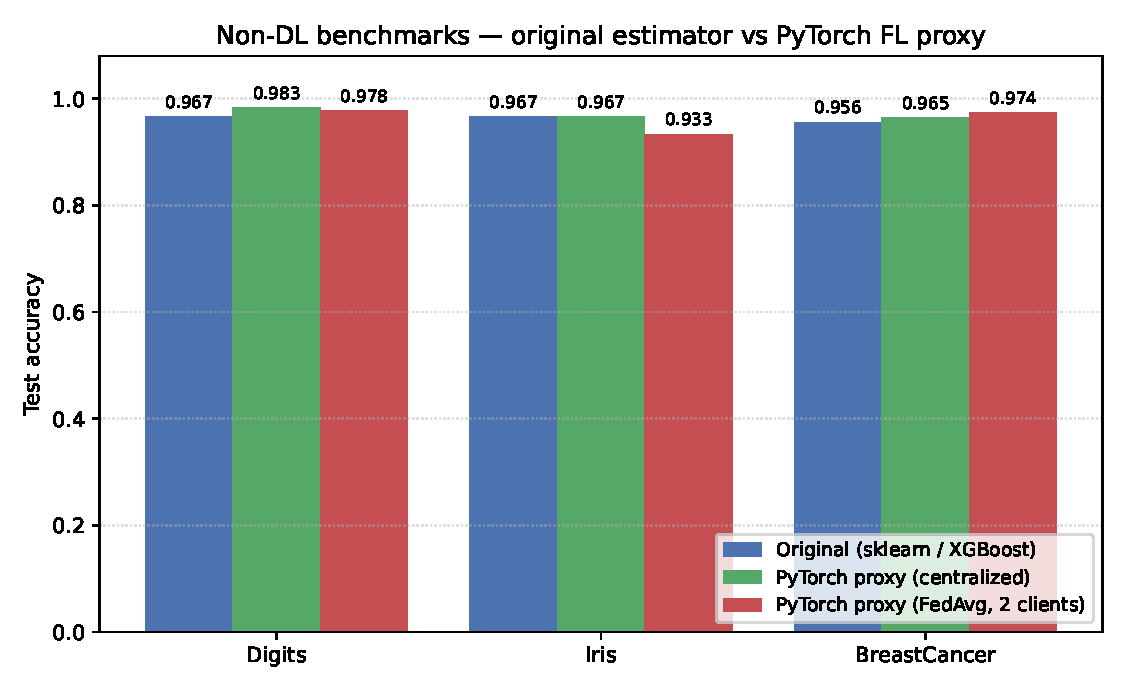
\includegraphics[width=0.85\linewidth]{results/figures/fig8_non_dl_validation.pdf}
  \caption{Test accuracy of the original non-DL estimator (sklearn /
    XGBoost) versus the PyTorch FL proxy in centralized and two-client
    FedAvg modes. The proxy preserves the original estimator's accuracy
    on all three benchmarks, supporting the semantic validity of the
    non-DL FL extension.}
  \label{fig:non_dl_proxy}
\end{figure}
